%%%%%%%%%%%%%%%%%%%%%%%%%%%%%%%%%%%%%%%%%%%%%%%%%%%%%%%%%%%%%%%%%%%%%%%%%%%%
% AGUJournalTemplate.tex: this template file is for articles formatted with LaTeX
%
% This file includes commands and instructions
% given in the order necessary to produce a final output that will
% satisfy AGU requirements, including customized APA reference formatting.
%
% You may copy this file and give it your
% article name, and enter your text.
% guidelines and troubleshooting are here: 

%% To submit your paper:
%% NOTES:
% DON'T USE SUBFIGURES!!!!

\documentclass[12pts,draft]{AR_analysis_}
% \usepackage{hyperref} % creates a hyperlink to the figure referenced
\usepackage{url} %this package should fix any errors with URLs in refs.
\usepackage{lineno}
%for better track changes. finalnew option will compile document with changes incorporated.
\usepackage[inline]{trackchanges}
\usepackage{soul}
\usepackage{float}  % Required for the [H] option
\usepackage{graphicx} % for my graphics
\usepackage{xcolor} % for my graphics
\usepackage{textcomp} % removes warning in gensymb
\usepackage{gensymb} % for basic symbols like degree
\usepackage{mathtools}
\usepackage{amsmath}
\usepackage{tabularx}
\usepackage{booktabs}
\usepackage{url}
%\usepackage{subcaption}

\usepackage{makecell}
\usepackage{array}

\newcolumntype{R}[1]{>{\raggedleft\arraybackslash}m{#1}}

% Bottom four packages from matplotlib -> LaTeX 
% Tutorial
% https://blog.timodenk.com/exporting-matplotlib-plots-to-latex/
\usepackage{tikz}
\usepackage{tikz-cd}
\usepackage{pgfplots}
\pgfplotsset{compat=1.14}

\linenumbers

%%%%%%%
% As of 2018 we recommend use of the TrackChanges package to mark revisions.
% The trackchanges package adds five new LaTeX commands:
%
%  \note[editor]{The note}
%  \annote[editor]{Text to annotate}{The note}
%  \add[editor]{Text to add}
%  \remove[editor]{Text to remove}
%  \change[editor]{Text to remove}{Text to add}
%
% complete documentation is here: http://trackchanges.sourceforge.net/
%%%%%%%

\draftfalse

%% Enter journal name below.
%% Choose from this list of Journals:
%
% JGR: Atmospheres
% JGR: Biogeosciences
% JGR: Earth Surface
% JGR: Oceans
% JGR: Planets
% JGR: Solid Earth
% JGR: Space Physics
% Global Biogeochemical Cycles
% Geophysical Research Letters
% Paleoceanography and Paleoclimatology
% Radio Science
% Reviews of Geophysics
% Tectonics
% Space Weather
% Water Resources Research
% Geochemistry, Geophysics, Geosystems
% Journal of Advances in Modeling Earth Systems (JAMES)
% Earth's Future
% Earth and Space Science
% Geohealth
%
% ie, \journalname{Water Resources Research}

\journalname{Geophysical Research Letters}

\begin{document}

%%%%%%%%%%%%%%%%%%%%%%%%%%%%%%%%%%%%%%%%%%%%%%%
%  TITLE
%
% (A title should be specific, informative, and brief. Use
% abbreviations only if they are defined in the abstract. Titles that
% start with general keywords then specific terms are optimized in
% searches)
%
%%%%%%%%%%%%%%%%%%%%%%%%%%%%%%%%%%%%%%%%%%%%%%%

\title{Influence of Atmospheric Rivers on Alaskan River Ice}

%%%%%%%%%%%%%%%%%%%%%%%%%%%%%%%%%%%%%%%%%%%%%%%
%
%  AUTHORS AND AFFILIATIONS
%
%%%%%%%%%%%%%%%%%%%%%%%%%%%%%%%%%%%%%%%%%%%%%%%

% Authors are individuals who have significantly contributed to the
% research and preparation of the article. Group authors are allowed, if
% each author in the group is separately identified in an appendix.)

% List authors by first name or initial followed by last name and
% separated by commas. Use \affil{} to number affiliations, and
% \thanks{} for author notes.
% Additional author notes should be indicated with \thanks{} (for
% example, for current addresses).

\authors{Russ Limber\affil{1, 2}, Elias C. Massoud\affil{2}, 
Jitendra Kumar\affil{2}, Bin Guan\affil{3, 4}, Forrest M. Hoffman\affil{2}}
\affiliation{1}{The University of Tennessee, Knoxville, Knoxville, TN, USA}
\affiliation{2}{Oak Ridge National Laboratory, Oak Ridge, TN, USA}
\affiliation{3}{Joint Institute for Regional Earth
System Science and Engineering, University of California,
Los Angeles, Los Angeles, CA, USA}
\affiliation{4}{Jet Propulsion Laboratory, California Institute
of Technology, Pasadena, CA, USA}

%(repeat as many times as is necessary)

% Corresponding author mailing address and e-mail address:

% (include name and email addresses of the corresponding author.  More
% than one corresponding author is allowed in this LaTeX file and for
% publication; but only one corresponding author is allowed in our
% editorial system.)

% Example: \correspondingauthor{First and Last Name}{email@address.edu}
\correspondingauthor{Russ Limber}{r62@ornl.gov}


%%%%%%%%%%%%%%%%%%%%%%%%%%%%%%%%%%%%%%%%%%%%%%%
% KEY POINTS
%%%%%%%%%%%%%%%%%%%%%%%%%%%%%%%%%%%%%%%%%%%%%%%
%  List up to three key points (at least one is required)
%  Key Points summarize the main points and conclusions of the article
%  Each must be 140 characters or fewer with no special characters 
% or punctuation and must be complete sentences

% Example:
% \begin{keypoints}
% \item	List up to three key points (at least one is required)
% \item	Key Points summarize the main points and conclusions of the article
% \item	Each must be 140 characters or fewer with no special 
	% characters or punctuation and must be complete sentences
% \end{keypoints}

% These are all under 140 characters
\begin{keypoints}

\item Interannually, atmospheric rivers (ARs) can lead to a week-long persistent 
	increase in daily air temperatures over Interior Alaska (AK)

\item In AK, ARs account for 36\% of annual precipitation, 57\% of extreme 
	precipitation and explain 48\% of interannual variability of precipitation

\item AR events during the coldest months delay the annual breakup date of 
	river ice, while ARs closer to the breakup date have less impact.

\end{keypoints}

%%%%%%%%%%%%%%%%%%%%%%%%%%%%%%%%%%%%%%%%%%%%%%%
%
%  ABSTRACT and PLAIN LANGUAGE SUMMARY
%
% A good Abstract will begin with a short description of the problem
% being addressed, briefly describe the new data or analyses, then
% briefly states the main conclusion(s) and how they are supported and
% uncertainties.

% The Plain Language Summary should be written for a broad audience,
% including journalists and the science-interested public, that will not have 
% a background in your field.
%
% A Plain Language Summary is required in GRL, JGR: Planets, JGR: Biogeosciences,
% JGR: Oceans, G-Cubed, Reviews of Geophysics, and JAMES.
% see http://sharingscience.agu.org/creating-plain-language-summary/)
%
%%%%%%%%%%%%%%%%%%%%%%%%%%%%%%%%%%%%%%%%%%%%%%%

%% \begin{abstract} starts the second page
%% The Abstract should be a single paragraph of fewer than 250 words
%% (for Geophysical Research Letters, under 150 words). 

\begin{abstract}
	
	Atmospheric rivers (ARs) transport vast amounts of moisture 
	from low to high latitude regions. One region particularly 
	impacted by ARs is Interior Alaska (AK). We analyze the impact 
	of ARs on the annual river ice breakup date for 25 locations 
	in AK. We investigate the AR-driven rise in local air temperatures 
	and explore the relationship between ARs and precipitation, 
	including extremes and interannual variability. We found that 
	AR events lead to an increase in local air temperatures
	for up to one week (by $\mathrm{\approx 1~\degree C}$). 
	Interannually, ARs account 
	for 36\% of total precipitation, explain 48\% of precipitation 
	variability, and make up 57\% of extreme precipitation events. 
	By estimating the heat transfer between winter precipitation
	and the river ice surface, we 
	conclude that increased precipitation during the 
	coldest period of the year delays river ice breakup dates, 
	while precipitation occurring close to the breakup date has little 
	impact on breakup timing.

\end{abstract}

% The PLS should be a single paragraph no more than 200 words long.

\section*{Plain language summary}

	Atmospheric rivers (ARs) are large storm systems originating in
	tropical regions capable of depositing large amounts of
	precipitation in high latitude regions. 
	Using river ice breakup data recorded throughout Interior
	Alaska (AK) we set out to explore the relationship between
	ARs and annual river ice breakup timing from 1980 to 2023. 
	We found that 
	daily air temperature increases can last up to
	one week after an AR event. Interannually, ARs
	account for 36\% of total precipitation, 
	explain 48\% of the variability of precipitation, and make up 57\% 
	of extreme precipitation events. We then
	approximated the total heat transfer between precipitation 
	and the river ice surface. We used the mass and temperature 
	of precipitation accumulated on the river ice surface to approximate 
	thermal energy exchange. The magnitude of energy exchange was then
	correlated to river ice breakup timing. We found that greater 
	amounts of precipitation from both AR and non-AR induced precipitation,
	occuring relatively close to
	river ice breakup dates, have little correlation to the breakup
	date. However, increased precipitation
	during the coldest period of the
	year (typically late December to early February) is strongly inversely
	correlated with river ice breakup timing and seems to delay
	the breakup date.

%%%%%%%%%%%%%%%%%%%%%%%%%%%%%%%%%%%%%%%%%%%%%%%
%
%  BODY TEXT
%
%%%%%%%%%%%%%%%%%%%%%%%%%%%%%%%%%%%%%%%%%%%%%%%

%%% Suggested section heads:
% \section{Introduction}
%
% The main text should start with an introduction. Except for short
% manuscripts (such as comments and replies), the text should be divided
% into sections, each with its own heading.

% Headings should be sentence fragments and do not begin with a
% lowercase letter or number. Examples of good headings are:

% \section{Materials and Methods}
% Here is text on Materials and Methods.
%
% \subsection{A descriptive heading about methods}
% More about Methods.
%
% \section{Data} (Or section title might be a descriptive heading about data)
%
% \section{Results} (Or section title might be a descriptive heading about the
% results)
%
% \section{Conclusions}



\section{Introduction}

Atmospheric rivers (ARs) are narrow corridors of intense water vapor
that significantly influence hydrologic events, transporting
most of the water vapor outside of the Tropics \cite{AR_def}.
It is estimated that ARs are responsible for as much as 90\% of poleward
water vapor transport at midlatitudes \cite{other_alg}. ARs contribute to
extreme precipitation events across various regions worldwide 
\cite{Espinoza2018, Massoud2019}, including
Western North America \cite{Dettinger2004, Neiman2008, Guan2010,
ARs_flood_WA_State, ARs_flood_Russian_River_CA, Ralph2013, ARs_CA}
Europe \cite{Lavers2013, ARs_impact_Norway}, the Middle East \cite{massoud2020, 
Lashkari2020, Esfandiari2024}, and Western South America
\cite{ARs_impact_SA}. In recent years, the impacts of ARs on the cryosphere
such as Greenland \cite{Mattingly2018} and Antarctica \cite{Gorodetskaya2014, 
Wille2021, Maclennan2022}, have been more extensively analyzed. 
In addition, a growing number of works 
investigating the relationship between ARs and 
high latitude regions have been undertaken 
\cite{Hegyi2018, Wang2024}. Evidence shows that between
1981 and 2020, higher atmospheric moisture content was significantly correlated
with lower sea ice coverage over almost the entire Arctic Ocean
\cite{ARs_lead_to_sea_ice_loss}. For those same years, another analysis
found that 100\% of extreme temperature events in the Arctic (above 0
$\mathrm{\degree C}$) coincide with the presence of 
ARs \cite{Ma2023}. Analyses have noted
a relationship between frequent AR activity and sea ice loss, caused by
increased rainfall from moisture originating in lower latitudes
\cite{Zhang2023, maclennan_contribution_2022}. However, Arctic systems
are complicated, as the intense moisture transport within ARs can also
result in heavy snowfall events, thus contributing to the accumulation
of snowpack, especially in mountainous regions \cite{Saavedra2020,
Guan2010}. Under the right conditions, this relationship has been found
to actually increase the mass balance of glaciers.
\citeA{Little2019} found ARs to be the primary drivers of both highest
ablation and snowfall events, substantially impacting glacier mass
balance at Brewster Glacier in New Zealand. 
Understanding the role of ARs in the cryosphere is essential for
assessing their broader impact on regional water resources and glacier
dynamics in a changing climate. 

While a number of works have explored
the relationship between ARs and sea ice, glaciers, and ice sheets, 
to our knowledge there has
been no study that investigates the relationship between ARs and Arctic
river ice. Past studies have used physics based processes
to model the annual breakup timing and conditions of Arctic river ice
\cite{Paily, ashton1986river, Prowse_Bonsal_Duguay_Lacroix_2007,
jasek1998, shen_newest}. Through such studies, it is recognized that an 
increase in precipitation leads to an increase in
streamflow, altering the hydraulics associated with river ice breakup, and 
potentially accelerating mechanical breakup events \cite{ashton1986river}.
It has also been proposed that increased snow pack as a result of increased 
precipitation contributes to breakup severity \cite{Prowes2002}. Using 
breakup records throughout Interior Alaska (AK) from the Alaska-Pacific 
River Forecast Center Database
(the same breakup records used in this analysis) \citeA{Bieniek2011} determined 
that winter precipitation plays a relatively minor role in impacting the 
breakup timing of river ice and if anything accelerates the breakup timing as a 
result of increased streamflow. They also report that 
increased storm activity in the spring leads to increased surface air 
temperature, leading to earlier breakup dates \cite{Bieniek2011}. However, 
their analysis used only 4 sites (as opposed to the 25 used in this analysis) 
and aggregated precipitation seasonally, without accounting for the interaction 
between winter precipitation and temperature that occurs at a finer temporal
resolution. 

Our analysis aims to answer the following questions: 
1.) Since ARs have been known to impact Arctic systems by increasing 
temperatures, is there a change in
air temperature in different regions of AK corresponding to the 
presence of ARs?
2.) How do ARs contribute to precipitation throughout AK, 
considering how ARs impact total annual precipitation, interannual 
variability, and extreme events?
3.) How do ARs impact the timing of river ice breakup, does the presence 
of ARs accelerate or delay the timing of river ice breakup?

\section{Data}

\subsection{Atmospheric Rivers Catalog}

Similar to previous studies, we define ARs using integrated vapor
transport (IVT) constructed from 6-hourly values of 3‐D wind and
water vapor at eight pressure levels between 300 and 1,000
mb from the National Center for Environmental Protection (NCEP) 
reanalysis data product \cite{NCEP_NCAR_reanalysis}. 
AR detection is based on version 3 of the tARget algorithm
\cite{Guan_Waliser2019, bin2022}.
The IVT values are calculated at the original
resolution from the NCEP
meteorological inputs \cite{NCEP_reanalysis}.
\citeA{alg_for_detecting_AR_moisture_fluxes} developed a global
AR detection algorithm, which was updated and validated later with
dropsonde data \cite{guan2018}. This algorithm is employed in
our study, which is based on a combination of IVT magnitude,
direction, and geometry characteristics, to objectively identify ARs.
Contiguous regions of enhanced IVT transport are first identified from
magnitude thresholding (i.e. grid cells above the seasonally
and locally dependent $85^{\text{th}}$ percentile, or 
$\mathrm{100\frac{kg}{m*s}}$, 
whichever is greater) and further filtered
using directional and geometry criteria requirements. Although the 
$\mathrm{100\frac{kg}{m*s}}$ threshold is applied globally, it is intended for 
dry (including polar) regions since in other regions the $85^{\text{th}}$ percentile 
is already larger than $\mathrm{100\frac{kg}{m*s}}$. The detection
algorithm was applied to NCEP reanalysis data at its native resolution of $2.5 \degree$.
This detection algorithm had over 90\% agreement in detecting AR
landfall dates when compared with other AR detection methods for Western
North America \cite{Neiman2008}, the United Kingdom \cite{Lavers2011}, 
and East Antarctica \cite{Gorodetskaya2014}. 

\subsection{Daymet Daily Surface Weather and Climatological Summaries}

Daily minimum ($T_{\text{min}}$) and maximum ($T_{\text{max}}$) temperatures and 
precipitation data were obtained from Daymet \cite{Daymet}. 
Daymet provides continuous and gridded estimates of daily weather at
$\mathrm{1km \times 1km}$ resolution. Daymet precipitation, 
$T_{\text{min}}$ and $T_{\text{max}}$, were selected in this analysis
due to their strong agreement with NCEP temperature time series for our 
region of interest (Figure \ref{fig:maps_crooked_creek}C). 
Daymet is derived by interpolating and extrapolating from in situ instruments 
and meteorological stations, and represents a robust 
dataset for precipitation and temperature predictions across North
America \cite{daymet2021}. This dataset has been a standard for validation 
among several analyses related to arctic regions \cite{Diro2019, 
Akinsanola2024}. Figure~\ref{fig:maps_crooked_creek}
(A, B) show the annual mean precipitation and temperature for the year
2021 across Alaska. For one of the study locations, Crooked Creek at the
Kuskokwim River, Figure \ref{fig:maps_crooked_creek} (C)
shows the time series of precipitation, temperature and AR events for the
year 2021.

\begin{figure}
\centering
\includegraphics[width=1.0\textwidth]{./images/maps_crooked_creek.png}
	\caption{(A): map shows annual total precipitation for the
	year 2021. (B): map of average daily temperature for 2021. (C):
	One of the 25 locations (Crooked Creek on the Kuskokwim
	River) for the year 2021. Yellow, orange, red represent the
	temperature profiles (fill plot of $T_{\text{min}}$ -
	$T_{\text{max}}$) from NCEP
	temperature data at 850, 925 and 1000mb respectively. Light
	green represents the Daymet temperature profile. Dark blue line shows
	precipitation from Daymet ($\mathrm{\frac{kg}{m^{2}}}$) 
	relative to the secondary y-axis in dark blue
	on the right. The light blue stem
	plots depict the IVT of AR events ($\mathrm{\frac{kg}{m*s}}$) 
	relative to the secondary y-axis in light blue
	on the right. The vertical purple dashed line shows the breakup
	date for the Kuskokwim River in 2021 for Crooked Creek.}
\label{fig:maps_crooked_creek} 
\end{figure}

\subsection{River ice breakup observations}

Observations for river ice breakup dates 
were obtained from the Alaska-Pacific River Forecast Center database.
While exact coordinates were unavailable, location coordinates
were estimated based on proximity to weather stations and airports, to 
maintain spatial consistency with inputs used in Daymet’s meteorological 
models. We identified 25 locations (shown in Figure 
\ref{fig:maps_crooked_creek} (A, B)) in the database that had
at least 35 breakup records between 1980 and 2023 
(the current temporal availability of 
Daymet), although breakup records go as far back as 1896 for some 
locations. The 35 breakup records threshold was used because it 
allowed for the greatest 
number of locations with the most complete time series 
necessary for statistical analysis. There is always one breakup 
date per year, but not every year had a recorded date, so some 
years are represented as empty values in the dataset. On average, 
recorded breakup dates range from mid-March to late-June 
This dataset has been used in several other studies such as 
\cite{murphy2022, Brown2018, Bieniek2011}. As an example, 
the breakup date for Crooked Creek 
at the Kuskokwim River in 2021 occurred in early-May and
is depicted in Figure 
\ref{fig:maps_crooked_creek} (C) with a 
vertical purple dashed line.



\section{Methods}

To assess the influence of ARs on local temperature, we analyze 
the relationship between the presence of an AR and the temperature 
change at a specific location. The presence of an AR is represented 
numerically as a binary value indicating whether or not an AR is 
active on a particular date. We then estimate how many days this 
change in temperature persists. To do this, we conducted a pairwise
\emph{t}-test using a varying temporal window.
In other words, for each
AR occurrence in the dataset, a pre--AR time window and post--AR
time window each equal to \emph{n}
days in length was created before and after the AR event date, respectively,
whereby: $ n \in \{1, 2, 3, \ldots, 14\}$.
For values of \emph{n} greater than one day the mean was 
calculated within each time window
for $T_{\text{min}}$ and $T_{\text{max}}$. These averaged 
temperatures were then
calculated over all locations. Mean temperature pairs 
were assessed using a one tailed pairwise \emph{t}-test to check
whether ARs increased the local temperature over period of 
time \emph{n} $(\alpha =
0.05)$. For example, if $\emph{n} = 3$ assessing $T_{\text{min}}$,
then the mean of $T_{\text{min}}$ three days prior to each AR event
will be compared to the mean of $T_{\text{min}}$ for
the three days post each AR event.

%We explored how ARs contribute to precipitation, by
%separating AR-based precipitation from the total precipitation amount.
We explored AR contribution to precipitation by seperating precipitation
events occuring on days with an active AR.
We then used the Wilcoxon rank-sum test \cite{Rey2011} to test 
the hypothesis 
that AR events tend to produce more precipitation than other
precipitation events. We opted to use a non-parametric 
test (Wilcoxon rank-sum test) 
because the distributions of precipitation were shown to
not be normal after log transformation using the
Shapiro-Wilks test \cite{shapiro_wilk_test}. We also estimated
the interannual variability of precipitation associated with ARs by
conducting a univariate ordinary least squares regression (OLS). 
For extremes, we extracted the top 5\% of precipitation events and determined 
what fraction of those events occured on days with an active AR event. 

To determine the impact that ARs have on river ice breakup timing, 
we estimate the heat transfer between the river ice and 
the precipitation accumulating on the surface. 
Assuming presence of a frozen layer of ice on the river surface, we estimate
the sensible heat transfer between the river surface and incoming
precipitation using Equation \ref{eq:heat_transport}. Latent heat
transfer fluxes were assumed to be relatively small and thus 
ignored in our simplified 
heat transfer calculations. The specific heat of precipitation in Equation
\ref{eq:heat_transport} is represented as either water or liquid as determined 
by air temperature. Given that Alaska is at a high latitude with heat transfer
calculated during the coldest period of the year, it can be assumed that 
in most cases the precipitation is in the form of snow.


\begin{equation}
q_{t} = \rho \cdot m \cdot \Delta T 
	\label{eq:heat_transport}
\end{equation}

\noindent where $q_{t}$ is heat flux ($\mathrm{\frac{J}{m^2}}$) at a 
given day \emph{t}; 
$\rho$ the specific heat 
of the precipitation (assumed to be either water or 
snow depending on the temperature)
($\mathrm{\frac{J}{kg \degree C}}$); $\Delta T$ is the difference between 
the temperature of the precipitation which is approximated 
using $T_{\text{min}}$ as a proxy, and the river ice surface which is
assumed to be at 0 $\mathrm{\degree C}$; $m$ 
the mass of the precipitation per unit area ($\mathrm{\frac{kg}{m^{2}}}$). 

%\hl{The sum of these values
%for all precipitation events that occurred six months prior to the
%breakup date on a daily basis is calculated.}
Heat transfer fluxes were calculated as a daily series for a period of six
months prior to the breakup date. Time of occurrence and thermal
conditions associated with precipitation events during winter and spring
have differential impacts to reinforce versus weaken the river ice layer and
thus the date of the breakup.  
We fit a temporal bias function (Equation \ref{eq:cases}), a double
exponential function, applied to the heat transfer equation to assess 
the days of the year when precipitation events were more 
impactful on breakup timing. The bias function is a symmetric unimodal
exponential function to help identify the most influencial precipitation
time period determining the annual time of river ice breakup. This bias
function was fit individually for each of the study locations. 

\begin{equation}
	\label{eq:cases}
	f(t; \gamma, \kappa, DOY, c) =
	\begin{cases}
    	\frac{e^{-\gamma \cdot (-t - DOY)} - 1}{\kappa} & \text{if }
        	t < c \\
    	\frac{e^{-\gamma \cdot (t - DOY)} - 1}{\kappa} & \text{if }
        	t \geq c \\
	\end{cases}
\end{equation}

\noindent where $\gamma$ is a scale parameter impacting the width of
the exponential function; \emph{t} is time in days; 
\emph{DOY} is the Gregorian day of year
that the breakup date occurred; 
\emph{c} is a location parameter dictating the
center placement of the function; $\kappa$ is a normalizing constant.
Finally, Equation \ref{eq:final_eq} solves for $Q_{\text{year, location}}$,
the total thermal 
energy exchange for a given location, for a given breakup year.
Equation \ref{eq:final_eq} is tuned over the entire 
hyperparameter search space for each
location and each breakup year, optimized by selecting the 
parameter values that produce 
the Pearson correlation coefficient with the greatest absolute value. 
Here \emph{i} is the starting day of the time series approximately 
six months prior to the breakup date. 

\begin{equation}
\label{eq:final_eq}
	Q_{\text{year, location}} = \sum_{t=i}^{t=DOY} f(t; \gamma, \kappa, DOY, c) \cdot q_{t}
\end{equation}


\section{Results} 

\subsection{Atmospheric rivers impact on temperature}

We applied the pairwise \emph{t}-test comparing pre--AR and post--AR
time windows of length \emph{n} at all locations. Figures
\ref{fig:large}A and \ref{fig:large}B show the change in \emph{p}-values for each
value of \emph{n} where the dashed lines represent the mean
\emph{p}-value across
the study locations and the filled color curved signifies the interquartile range (IQR). 
%For example, looking at $T_{\text{min}}$ (\ref{fig:large}A), 
%the light blue represents the $\mathrm{25^{th}}$ to the 
%$\mathrm{75^{th}}$ percentile or IQR of \emph{p}-values, while the blue-grey is 
%the $\mathrm{75^{th}}$ 
%percentile to the maximum \emph{p}-value given \emph{n}. Same is true for the 
%color transition of $T_{\text{max}}$ in Figure \ref{fig:large}B. 
Figure \ref{fig:large}C and \ref{fig:large}D shows the mean increase 
in temperature from the pre--AR time window to the post--AR time window 
for varying time window sizes \emph{n}. 
%The mean
%temperature increase tends to be higher for $T_{\text{min}}$ post AR than  
%$T_{\text{max}}$, with both plots
%showing a clear downward trend as the length of \emph{n} 
%increases. 
%We found that there is a
%statistically significant difference in $T_{\text{min}}$ 
%(based on an $\alpha = 0.05$) roughly 8 days before and after 
%an AR event. 
Analysis shows an increase in air temperature during the period following an
AR event, with mean temperature increases higher for $T_{\text{min}}$
compared to $T_{\text{max}}$, with the difference receding over longer
time windows. On average, the temperature differences were statistically significant
for $T_{\text{min}}$ (based on an $\alpha = 0.05$) for temporal
windows up to 10 days after an AR event. For temporal
windows up to 7 days, statistical significance
was true for all locations within the study as represented
by the Figure \ref{fig:large}A fill plot.
The increase in daily minimum temperature can be as high as 1.5 
$\mathrm{\degree C}$ ($n=2$) (Figure \ref{fig:large}C). 
For $T_{\text{max}}$, the differences were statistically significant for up
to 6 days after an AR event on average (Figure~\ref{fig:large}B) with an increase
as high as 0.75 $\mathrm{\degree C}$ ($n={3, 4}$) (Figure~\ref{fig:large}D).
These statistically significant temperature increases following AR events
were true at all locations in our study for $n={2, 3, 4}$ as shown in
Figure \ref{fig:large}B fill plot. 

%The \emph{t}-test for
% $T_{\text{max}}$ implies that the presence of an AR can increase 
% temperatures for roughly 6 days on average (Figure 
% \ref{fig:large}B), with an increase as high 
% as 0.75 $\mathrm{\degree C}$ ($n={3, 4}$) (Figure 
% \ref{fig:large}D).    

\begin{figure}[H]
\centering
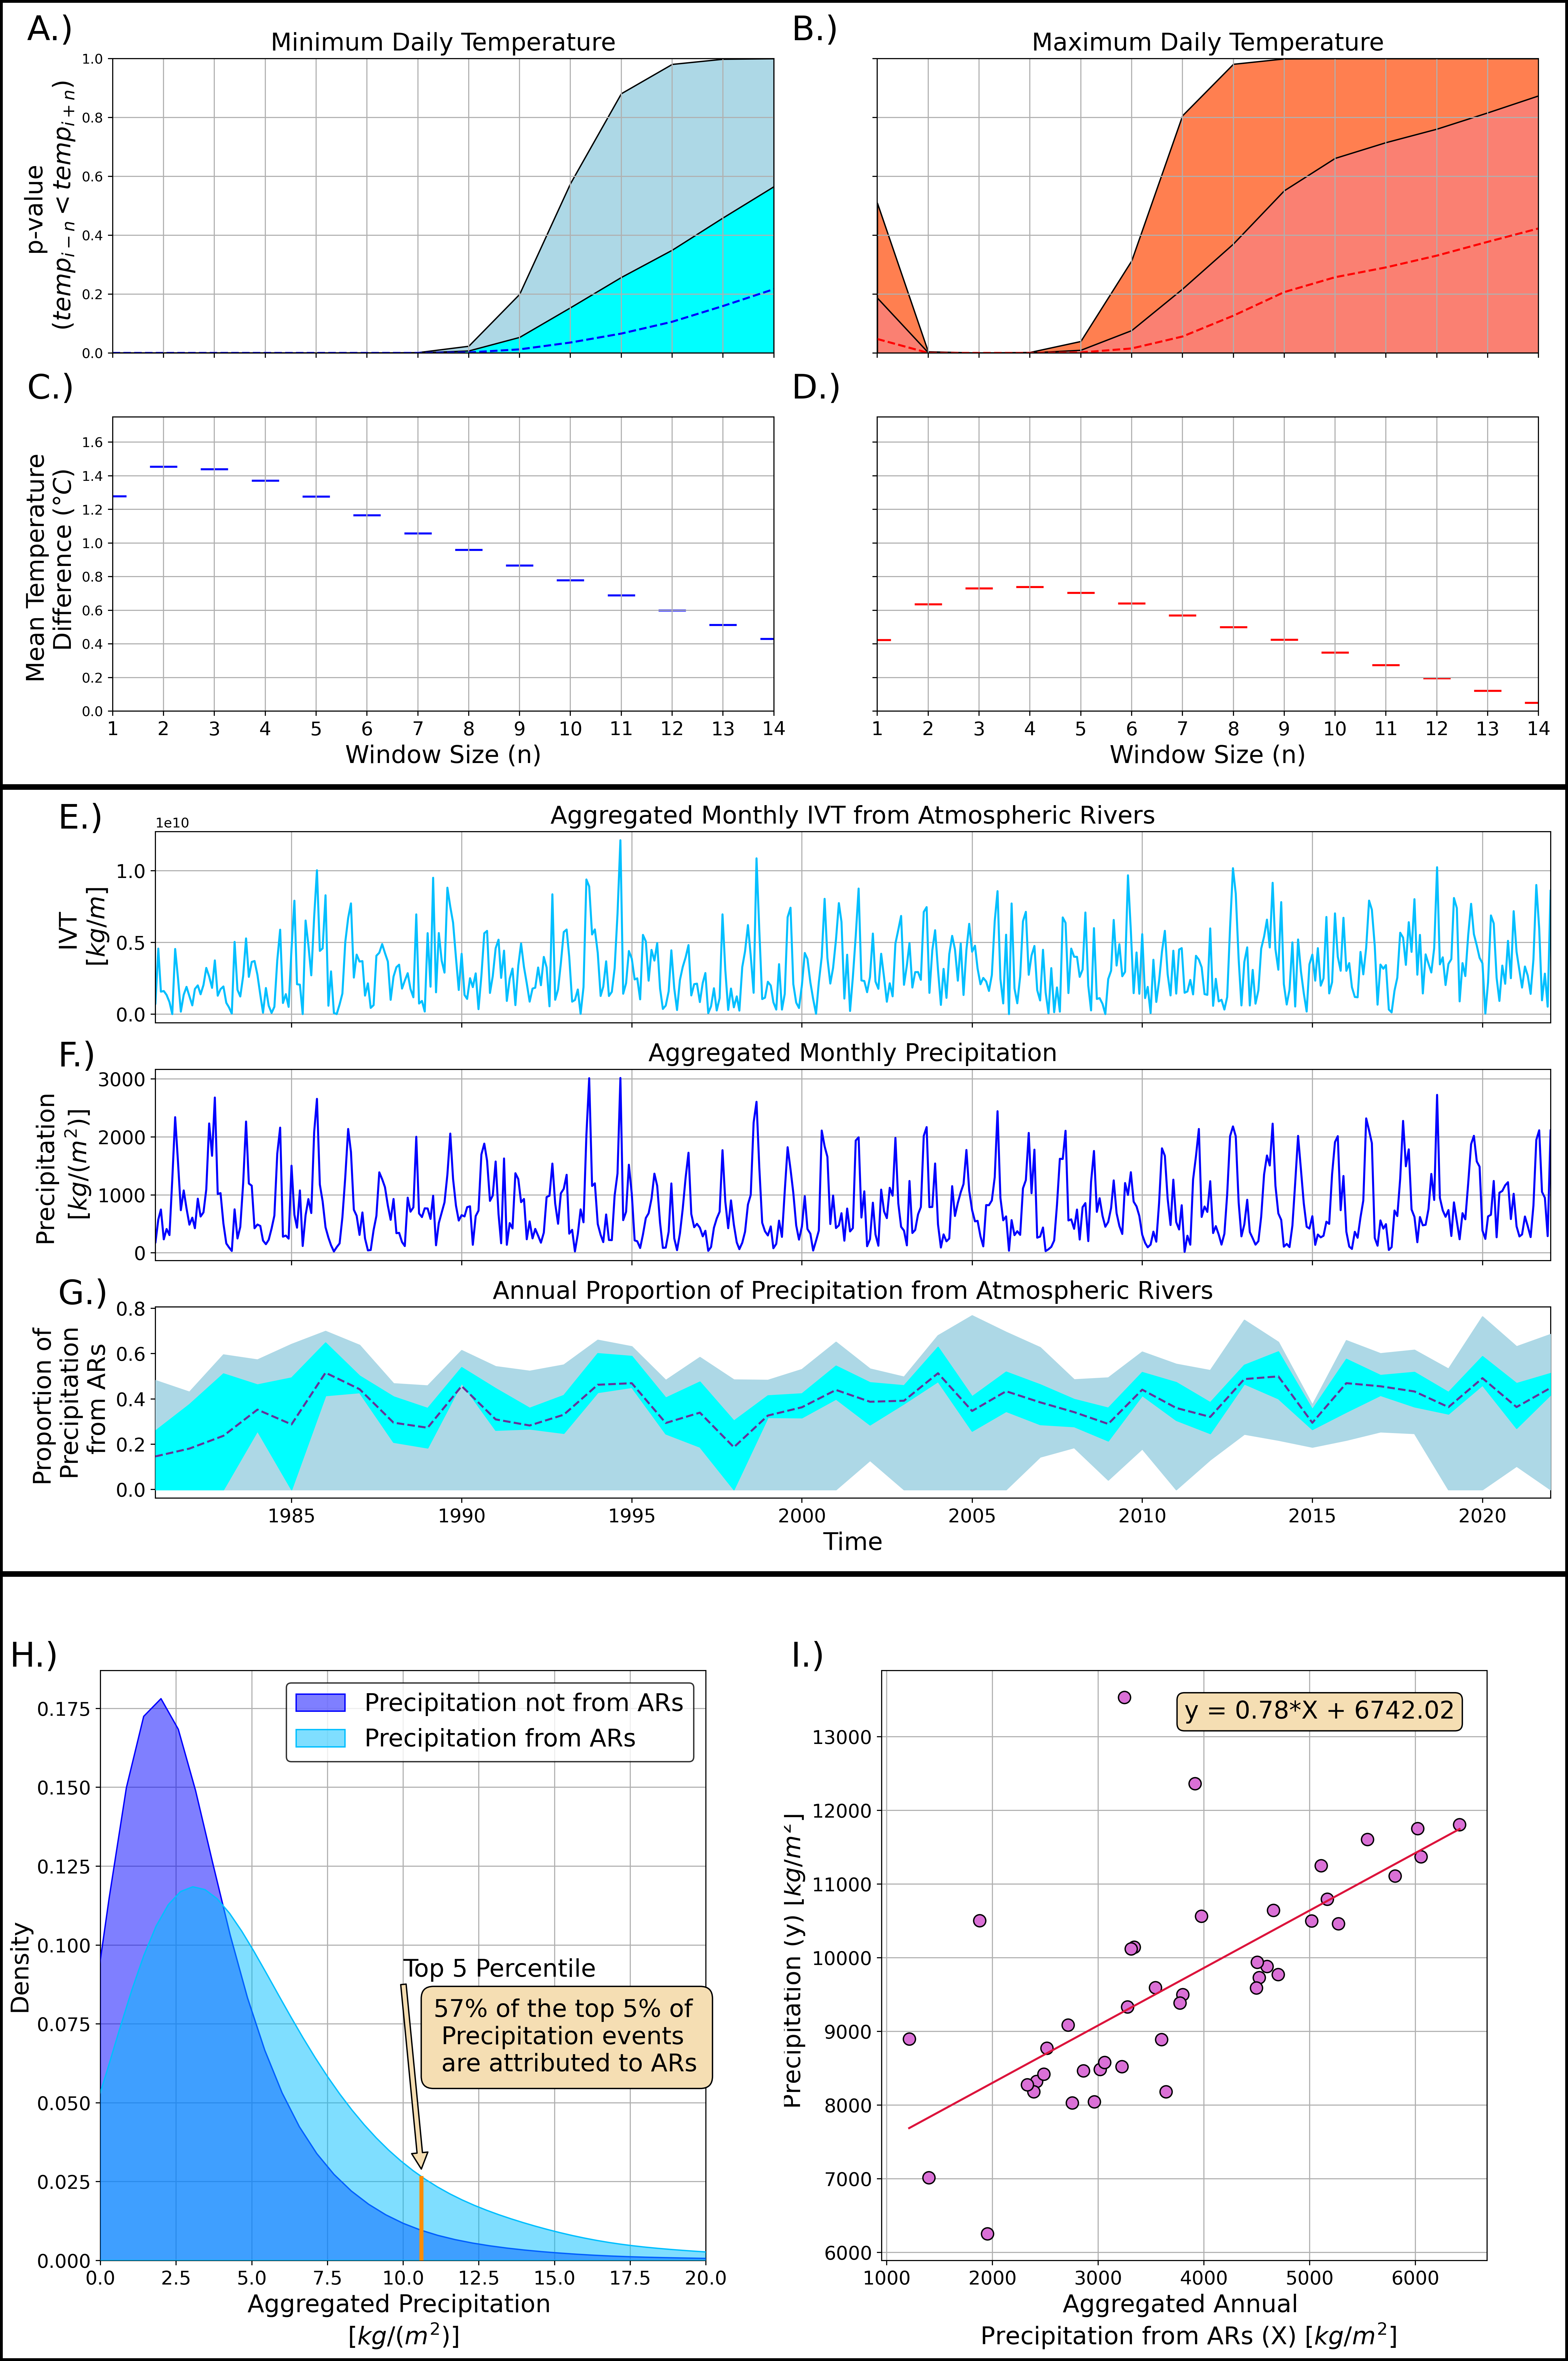
\includegraphics[width=0.8\textwidth]{./images/large.png}
\caption{(A and B): \emph{p}-values from the paired \emph{t}-test given
	time window size (\emph{n}) surrounding the AR event date (A:
	$T_{\text{min}}$; B: $T_{\text{max}}$). Dashed lines represent the
		mean, while the filled color curves show interquartile range
		(25th and 75th percentile); 
	(C and D): mean increase in temperature ($\mathrm{\degree C}$) 
	accompanying each AR, calculated between the pre--AR 
	time window and the post--AR time window 
	(C: $T_{\text{min}}$; D: $T_{\text{max}}$).
	(E): time series of IVT $\mathrm{\frac{kg}{m}}$ aggregated monthly 
	over all locations.
	(F): time series of total precipitation $\mathrm{\frac{kg}{m^{2}}}$ 
	aggregated monthly over all study locations. 
	(G): proportion of precipitation accounted for by
	ARs on an annual basis. 
	(H): kernel density plots showing the distribution of
	local precipitation (dark blue) and precipitation from ARs
	(light blue). 
	(I): ordinary least squares regression plot
	using total annual precipitation from ARs, to predict total annual
	precipitation.}
	
	
\label{fig:large} 
\end{figure}

\subsection{Atmospheric rivers impact on precipitation}

Figures \ref{fig:large}E and \ref{fig:large}F show the monthly IVT from 
AR events and monthly total precipitation through the span of the 
data record, aggregated over all locations, respectively. Figure \ref{fig:large}G
shows the proportion of total annual precipitation occuring on days with
active ARs over time, where 
light blue depicts the IQR of proportions and blue-grey represents 
proportions outside of the IQR, across all 25 locations. The dashed line 
represents the mean proportion.
ARs tend to account for 36\% of
precipitation on average (Figure \ref{fig:large}G), 
with a high degree of variability across
years and locations. In 2005 and 2020 for example, nearly 
80\% of the total precipitation at some locations occured on days with
active AR events. The results 
from the Wilcoxon rank-sum test show that
precipitation during active ARs tends to be greater in magnitude than non-AR 
precipitation
($\text{test statistic} = -83.85; \text{ p-value} \approx 0.0)$. In addition,
we found that of the top 5\% of precipitation events by total rainfall, 57\%
occured during active ARs (Figure \ref{fig:large}H).
Correlating total precipitation from AR days, to total annual
precipitation using a univariate OLS, we find that the
coefficient of determination ($\mathrm{R^{2}}$) is equal to 0.48 (Figure 
\ref{fig:large}I). This indicates that ARs
explain about 48\% of interannual variability in precipitation, 
across all 25 locations.  

%\begin{figure}
%\centering
%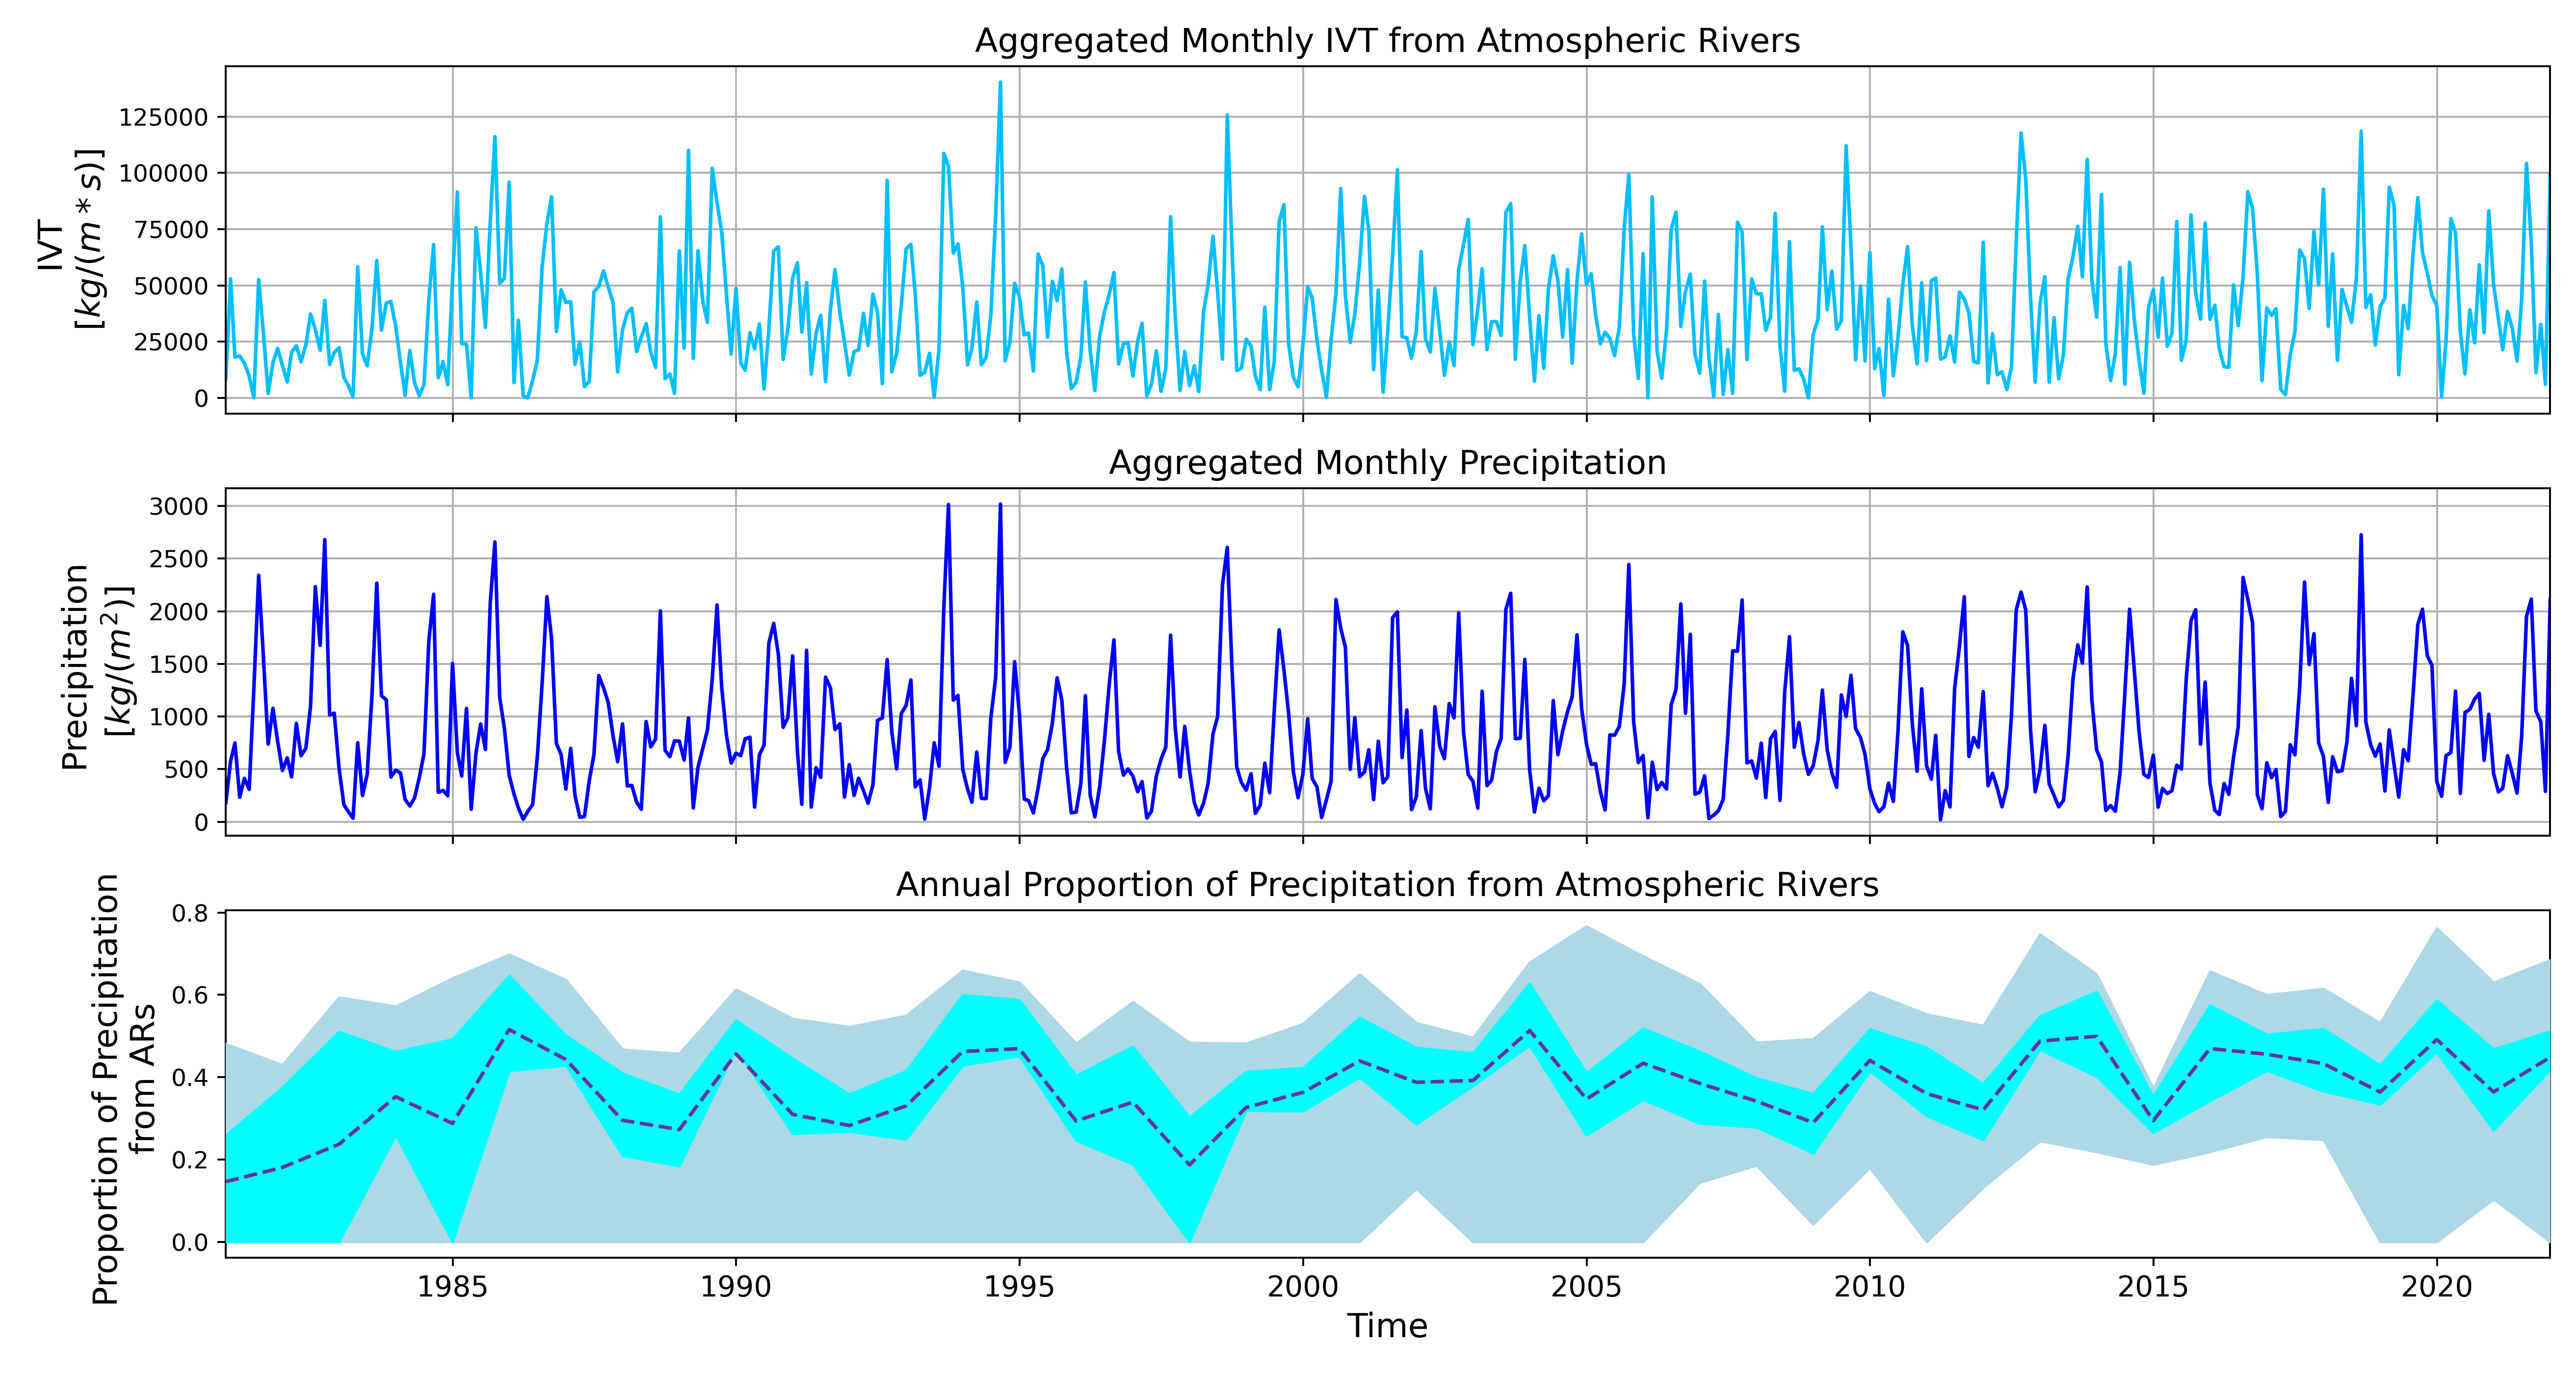
\includegraphics[width=1.0\textwidth]{./images/IVT_Precip_proportion_over_time.png}
%\caption{(A): time series of IVT $\mathrm{\frac{kg}{m}}$ aggregated monthly 
%	over all locations.
%	(B): time series of total precipitation $\mathrm{\frac{kg}{m^{2}}}$ 
%	aggregated monthly over all
%	locations. (C): proportion of precipitation accounted for by
%	ARs on an annual basis. Light blue depicts the $\mathrm{25^{th}}$ 
%	to $\mathrm{75^{th}}$
%	percentile (IQR) of proportion values, while the blue-grey represents 
%	proportions outside of the IQR, over all 25 locations. The dashed line 
%	represents the mean proportion.}
%\label{fig:IVT_Precip_proportion_over_time}
%\end{figure}

\subsection{Transfer of energy based on Precipitation}

To estimate the impact of precipitation on river ice breakup dates, we use 
Equation~\ref{eq:final_eq} to approximate the heat transfer
between precipitation and the river ice surface.
Equation~\ref{eq:final_eq} was solved using a double exponential bias
function to temporally-weigh events of higher influence 
(Figures~\ref{fig:concatenated_corr_plots}A, 
\ref{fig:concatenated_corr_plots}B, 
\ref{fig:concatenated_corr_plots}C), and using
uniform weights as baseline for comparison 
(Figures~\ref{fig:concatenated_corr_plots}D, 
\ref{fig:concatenated_corr_plots}E,
\ref{fig:concatenated_corr_plots}F).
When using a temporal bias function, the relationship between summated
heat transfer due to precipitation and time of river ice breakup were
identified with strong correlation (Pearson correlation coefficient
$(r_{p} )=$ -0.84 and a Spearman correlation coefficient
$(r_{s}) =$ -0.80 at Crooked Creek on the Kuskokwim river
(Figure \ref{fig:concatenated_corr_plots}A)).
In contrast, very weak correlations were identified when fitting the
relationship using temporally uniform weights (Figure
\ref{fig:concatenated_corr_plots}B), thus highlighting the need
for a temporal bias function. We tuned three different cases for 
Equation~\ref{eq:heat_transport} whereby the mass of precipitation 
could be provided by: total precipitation, precipitation from ARs or 
precipitation not from ARs. 
This exercise allows us to 
%estimate the energy input from \hl{local precipitation, 
%precipitation via ARs and total precipitation}, and 
determine whether or not that aggregated 
energy accelerates or decelerates the breakup of river ice. 
We find that there is a strong negative correlation between the heat 
transfer and the \emph{DOY} 
on which the river ice breakup occurs (Figure
\ref{fig:concatenated_corr_plots}A). In this context, negative values 
along the y-axis of Figures \ref{fig:concatenated_corr_plots}A and 
\ref{fig:concatenated_corr_plots}D 
are interpreted
as a negative heat exchange, suggesting a net cooling effect on the river ice
surface as the precipitation below freezing are accumulated
on the river ice surface. The
peak of the temporally-weighted bias curve is typically located during
the coldest period of the year, typically betweeen late November and
early February (Figure {\ref{fig:concatenated_corr_plots}}C).
In other words, the presence high magnitude precipitation events, occuring 
on colder days of the 
year, show a strong inverse correlation to the time of breakup. 
For example, referring to Figure \ref{fig:concatenated_corr_plots}A, 
Crooked Creek on the 
Kuskokwim River has a
clear negative trend, whereby the cooling effect of precipitation on the
river ice surface delays the \emph{DOY} of the breakup. 
%This
%relationship (based on Equation~\ref{eq:final_eq}) has a Pearson 
%correlation
%coefficient $ (r_{p} )=$ -0.84 and a Spearman correlation coefficient
%$(r_{s}) =$ -0.80 (Figure \ref{fig:concatenated_corr_plots}A). 
The frequency of AR events that occurred six months prior to
the breakup date alone is an insufficient predictor
(Figures~\ref{fig:concatenated_corr_plots}B,
\ref{fig:concatenated_corr_plots}E) of the breakup date. 

%The relationship between the total
%number of ARs that occurred in period six months prior to the breakup date and the
%\emph{DOY} are shown on the center column 
%(Figure \ref{fig:concatenated_corr_plots}B and 
%\ref{fig:concatenated_corr_plots}E; 
%these two plots are the same by
%definition) indicating that the number of AR 
%events that occur within the six months prior to the breakup
%is insufficient information 
%in correlating to breakup timing on its own. 

%The
%bottom row of Figure \ref{fig:concatenated_corr_plots} shows that the
%use of a bias function (Equation \ref{eq:cases}) is necessary, as simply 
%applying the summation of Equation \ref{eq:heat_transport} using an 
%equally weighted temporal bias function (the aggregated total heat 
%transfer) is uncorrelated. 

While Figure~\ref{fig:concatenated_corr_plots} focuses on a single
selected site, Table~\ref{tab:pearson} shows the Pearson correlation after
tuning parameters \emph{c} and $\gamma$ are optimized and applied to 
Equation 
\ref{eq:final_eq} individually at each location.
Table \ref{tab:pearson} also shows the center of the bias curve \emph{c} 
(month-day)
that was selected for, at each location, given the summand for 
precipitation used in
Equation \ref{eq:final_eq} (ie. Total Precipitation, Precipitation from ARs, 
Precipitation not from ARs; mulitplied to the temporal bias).  


%\begin{figure}
%\centering
%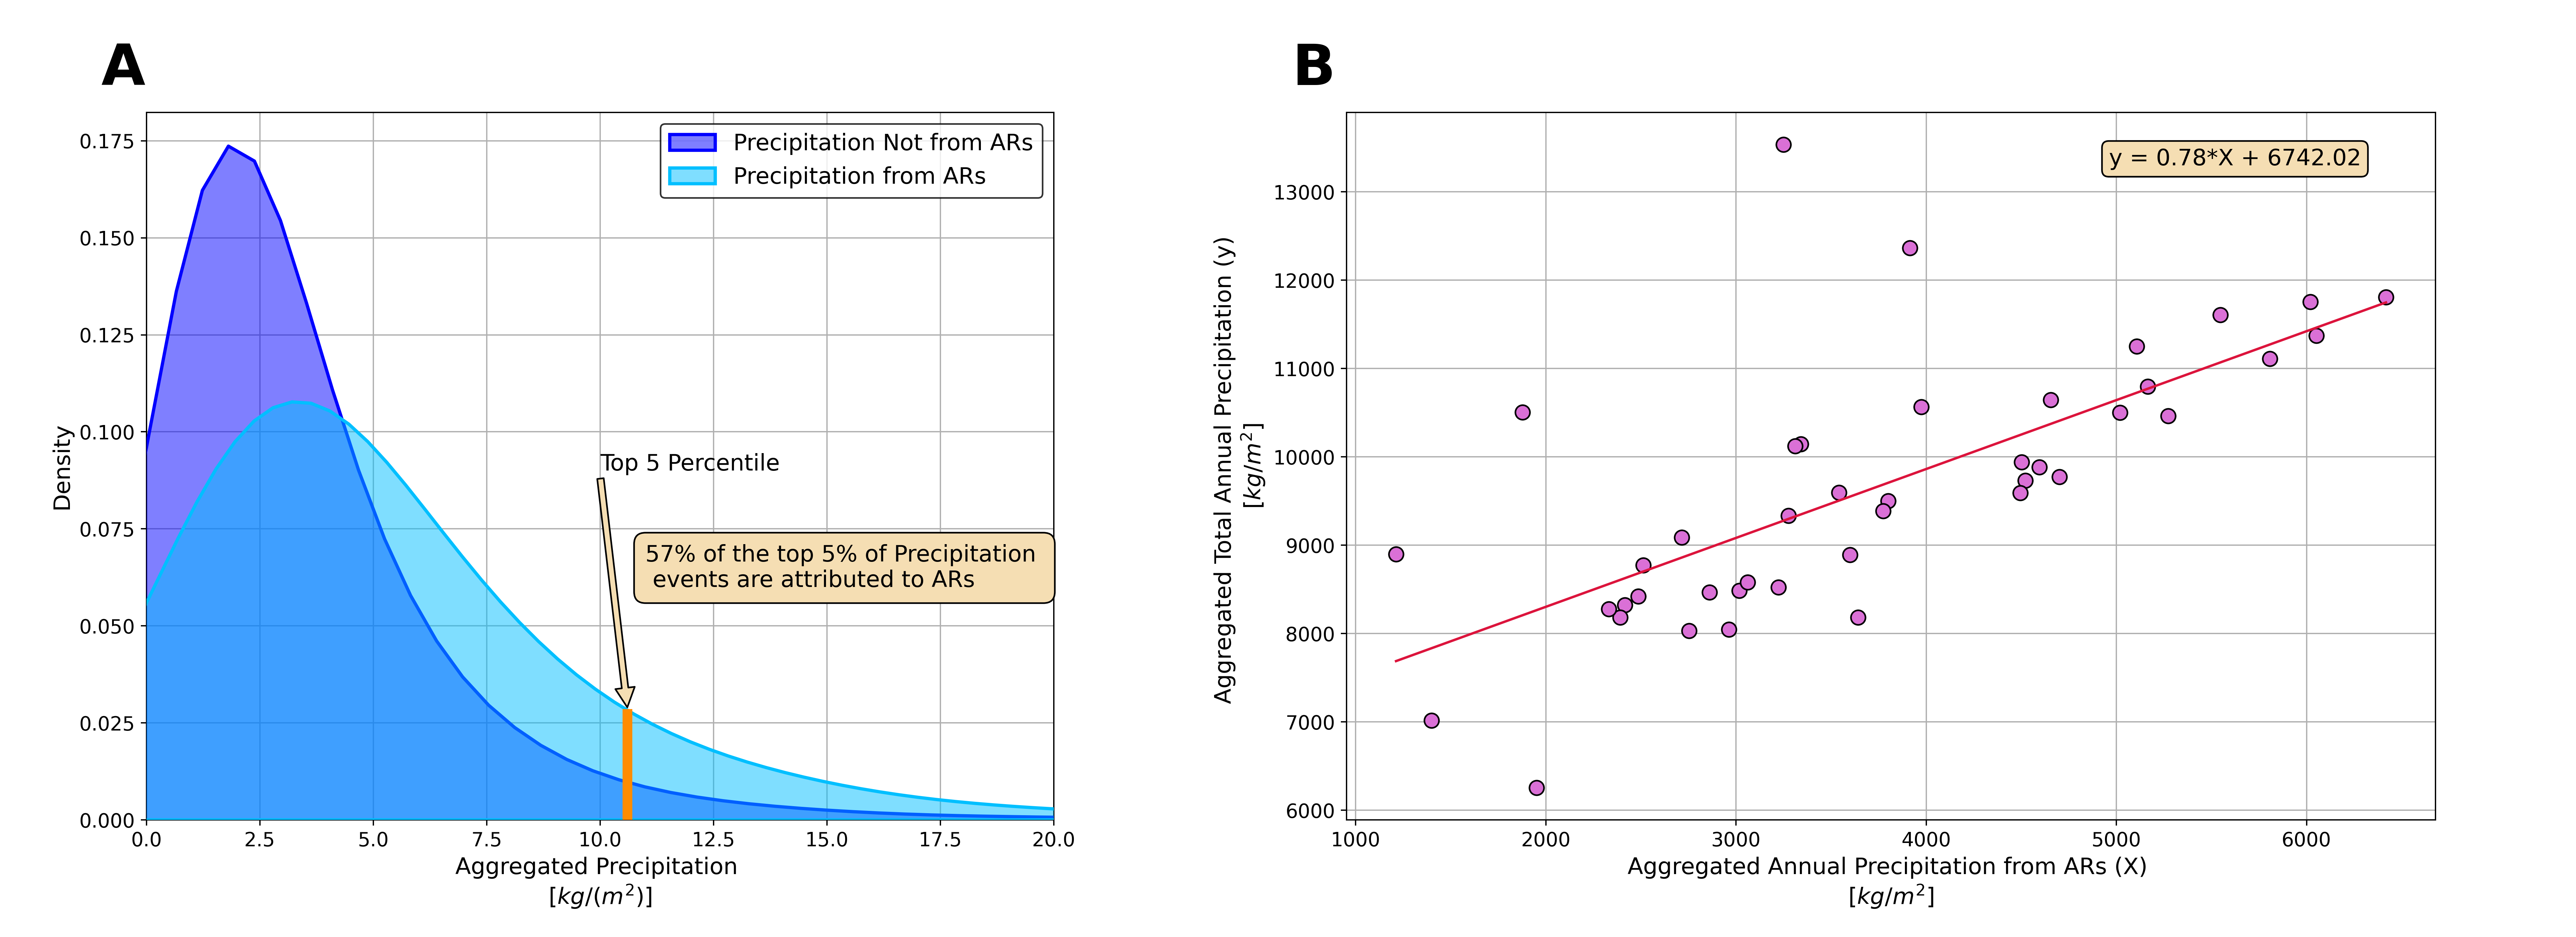
\includegraphics[width=1.0\textwidth]{./images/concatenated_precip_var_plots.png}
%\caption{(A): kernel density plots showing the distribution of
%	local precipitation (dark blue) and precipitation from ARs
%	(light blue). (B): ordinary least squares regression plot
%	using annual, summated precipitation from ARs, to predict total annual
%	summated precipitation.}
%\label{fig:concatenated_precip_var_plots}
%\end{figure}

\begin{figure}[H]
\centering
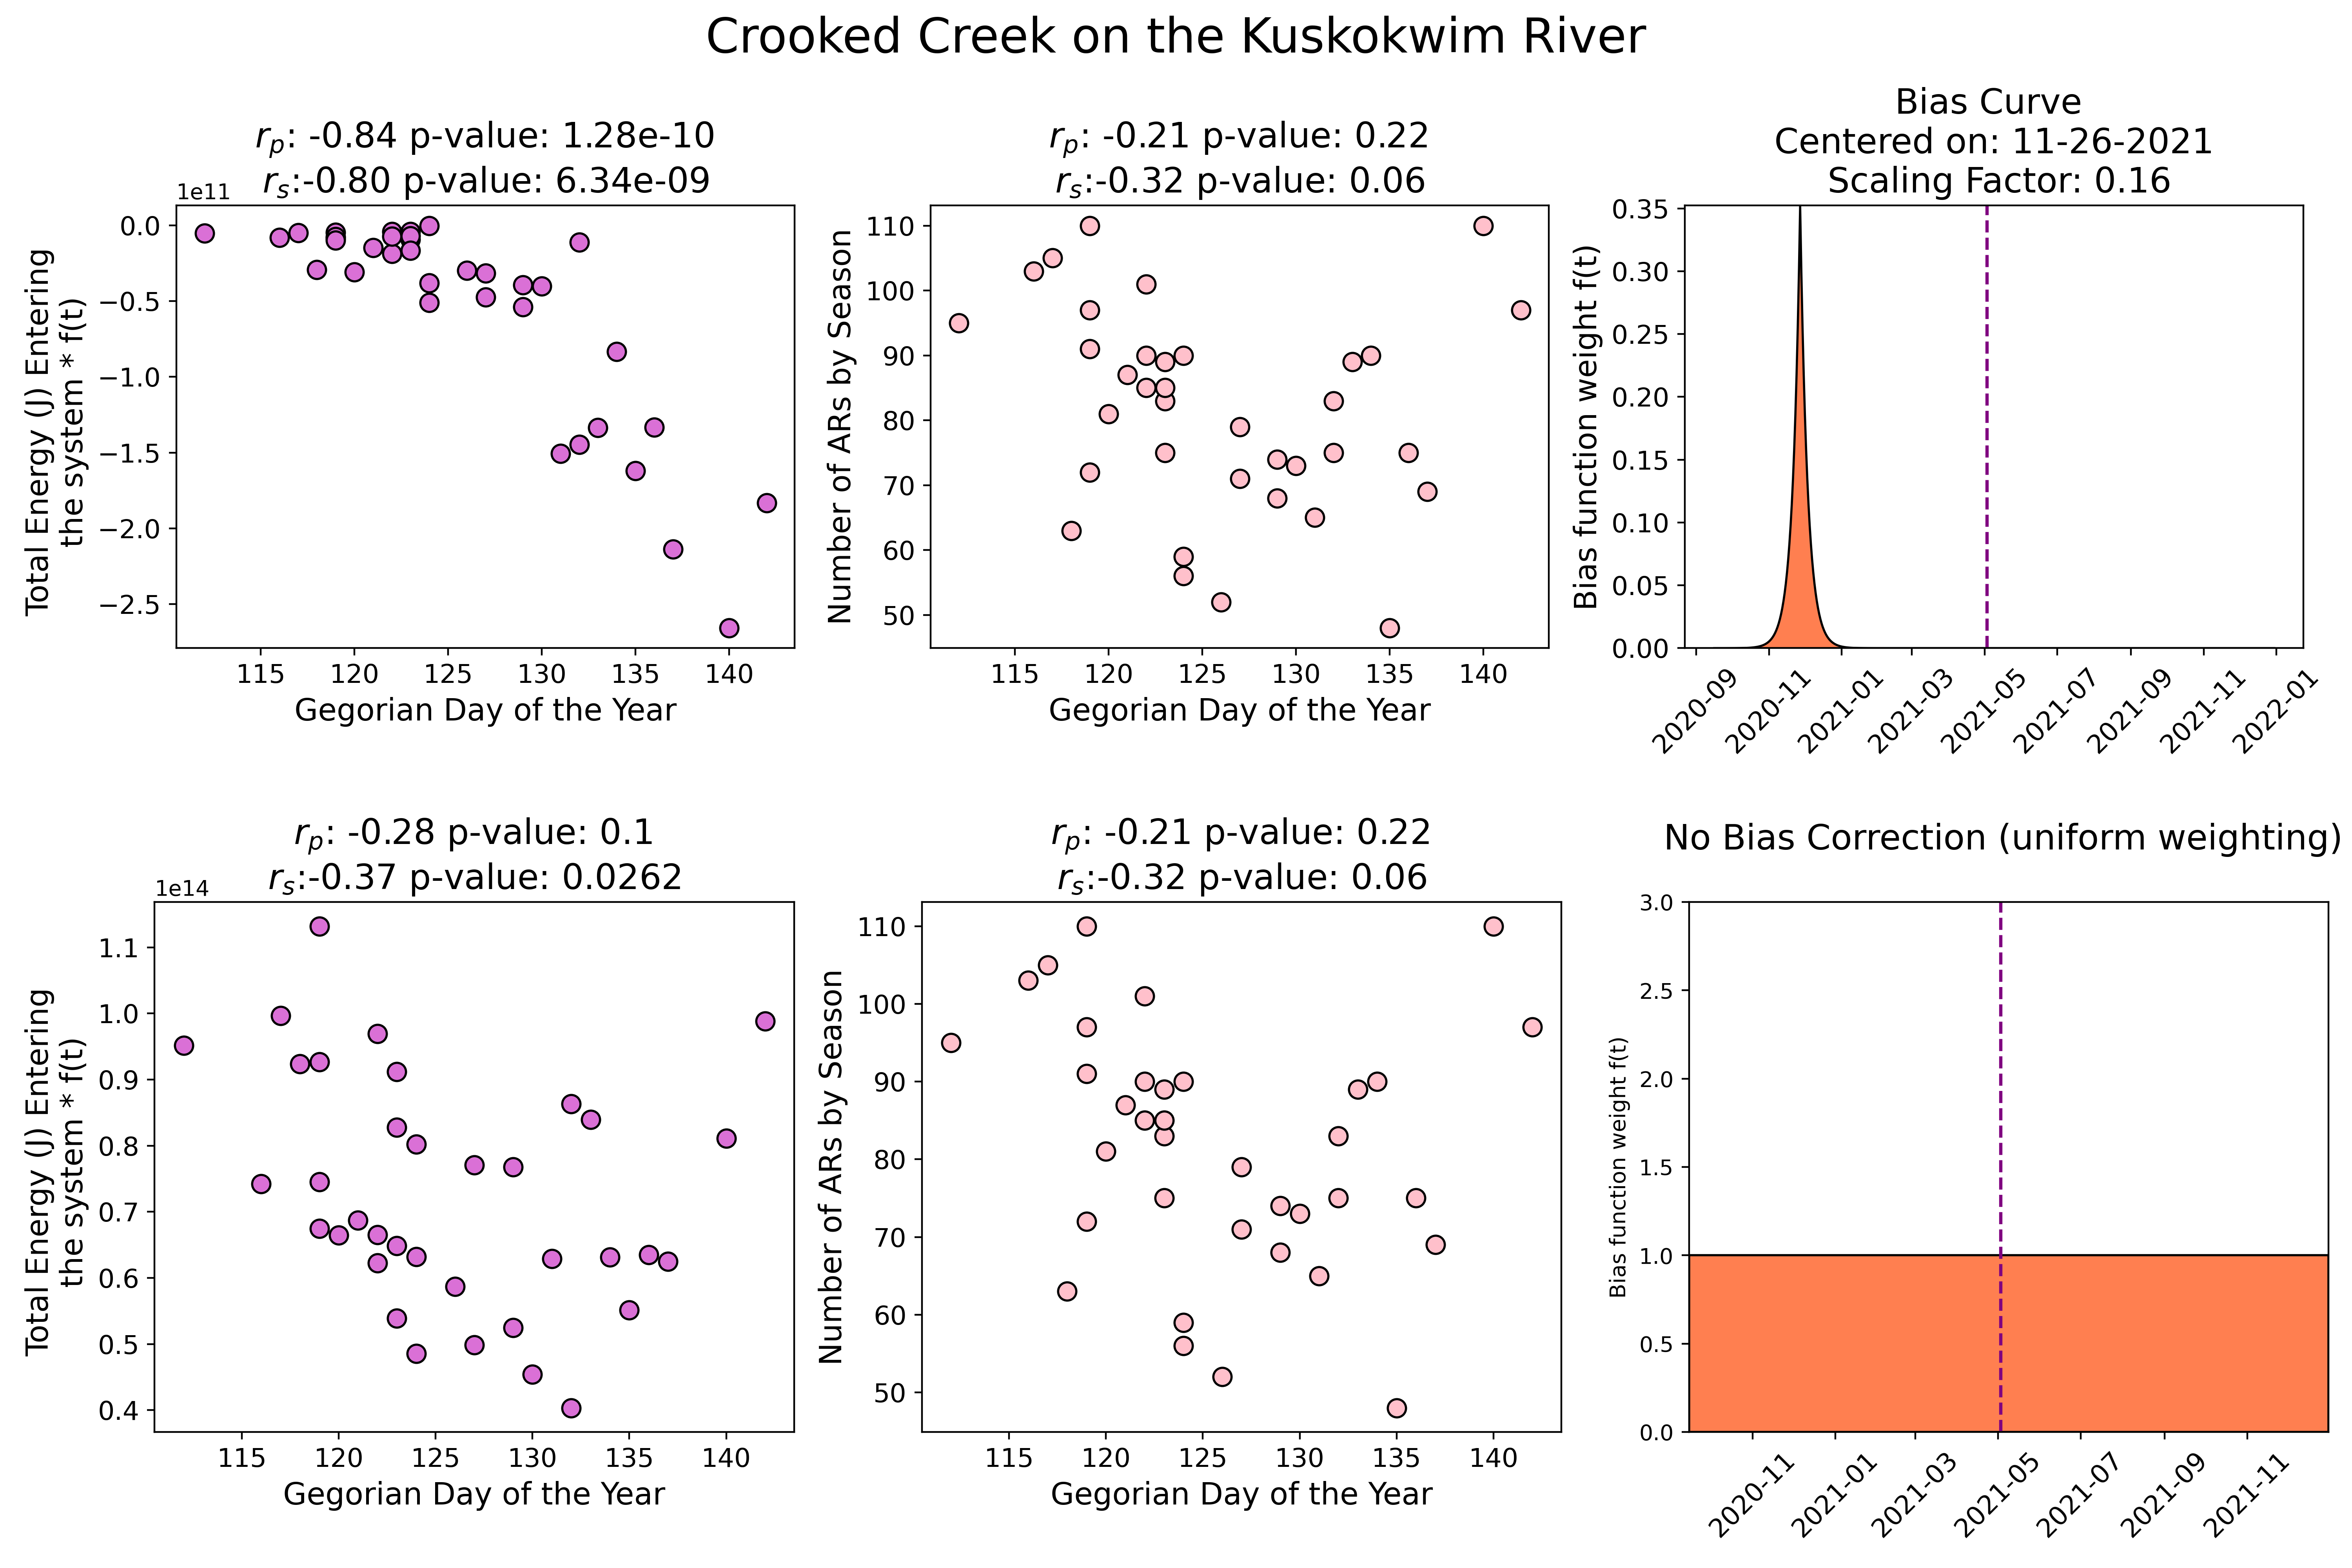
\includegraphics[width=1.0\textwidth]{./images/concatenated_scatter_bias_plots.png}
	\caption{top row: (A): scatter plot between thermal energy
	transfer for all precipitation events and \emph{DOY} (the Gregorian day 
	of year
	that the breakup date occurred); (B): scatter plot of the number of ARs
	that occured in the six months prior to the breakup date and
	\emph{DOY}; 
	(C): temporal bias curve for the year 2021 with the breakup
	date represented by the vertical dashed line. bottom row: same as
	the top row except depicting the results when a temporal bias
	is not utilized.}
\label{fig:concatenated_corr_plots}
\end{figure}



\section{Conclusion and Discussion}

This study investigated the impact atmospheric rivers (ARs) and 
non-AR related precipitation events have on the timing of river 
ice breakup across 25 sites in Alaska. 
We explored the impact of ARs on local temperature increases throughout 
the study domain; the contribution of ARs to precipitation events, 
including variability and extremes; and determined the impact of ARs and 
non-AR precipitation events on the \emph{DOY} 
on which the ice on the surface of Alaskan rivers eventually breaks. 

We found that ARs generally lead to up to a week-long persistent 
increase in daily temperature (minimum and maximum) across Alaska, with 
temperatures rising by as much as 1.5 $\mathrm{\degree C}$ 
for $T_{\text{min}}$ and 0.75 $\mathrm{\degree C}$ for $T_{\text{max}}$. 
These findings are consistent with  
many past studies that have shown that warm moisture and an increase 
in heat flux brought on by ARs can 
warm the cryosphere
\cite{Wille2021, Ma2023, ARs_lead_to_sea_ice_loss, Zhang2023}.
Our analysis also shows that ARs account for a significant portion of
total annual precipitation 
in Alaska, contributing to 36\% of total precipitation by volume on 
average. ARs also explain 48\% 
of interannual variability and lead to 57\% of extreme precipitation events 
(precipitation events within the top 5\% of deposition). These results are
consistent with past works, such as \citeA{Nash2024} which showed that 
throughout Southeast Alaska, as few as six annual AR events can account for 
68\% - 91\% of precipitation days. Our analysis shows evidence that intense 
ARs occurring during the coldest period of the year appear to delay the 
annual breakup date of river ice. Our results do not show that ARs are 
unique relative to non-AR forms of 
precipitation in this regard (Table \ref{tab:pearson}), with no evidence 
that increased 
precipitation events of any kind closer to the breakup date accelerates the 
breakup date.
This is likely attributed to a combination of heat transfer from 
precipitation, increased ice accumulation from the river ice precipitation
interface and structural changes in the river ice surface as a result 
of snowfall.
Increased snow accumulation
increases the albedo of the river surface, as well as provides thermal
insulation, mitigating the effects of temperature 
fluctuations during the coldest period of the year. This is 
consistent with the extensive analysis conducted by \citeA{Ashton2011}, 
showing that an increase in snow accumulation on the river ice surface 
for locations across Alaska (many of the same locations used in this 
analysis) can lead to 
an increase in river ice thickness, thus reinforcing the river ice 
structurally. This phenomenon is apparent to a point at which the efficacy 
begins to diminish. It should be noted that a limitation of
our analysis is the assumption that the river ice surface temperature is 
held constant at 0 $\mathrm{\degree C}$ and that air temperature is a 
reasonable proxy for
incoming precipitation. We were unable to 
find a complete dataset on river ice surface temperatures for the locations and time 
period of our study. Thus, we assume that the mass of liquid, snow or ice deposited on 
the river surface, times its temperature and specific heat, will be sufficient to
approximate the heat exchanged in the system.   

Understanding the influence of ARs and other HPEs on the
timing of river ice breakup in Alaska is 
crucial for predicting and managing the impacts of climate change in the region, 
especially since studies have shown that AR frequency and intensity in this region are 
expected to increase in a warmer world \cite{Espinoza2018, Massoud2019}. The findings 
of our analysis suggests that ARs have significant influence on the climate and
terrestrial hydrology across Alaska, 
affecting temperature, precipitation, and river ice dynamics. Further research in this 
area could help improve our understanding of ARs and their role in shaping the climate 
of high-latitude regions.


%%%%%%%%%%%%%%%%%%%%%%%%%%%%%%%%%%%%%%%%%%%%%%%
%
% DATA SECTION and ACKNOWLEDGMENTS
%
%%%%%%%%%%%%%%%%%%%%%%%%%%%%%%%%%%%%%%%%%%%%%%%

\section*{Data Availability Statement}
Daily Daymet precipitation and temperature data is available through the Oak Ridge 
National Laboratory Distributed Active Archive at \url{https://daymet.ornl.gov/single-pixel/}.
The National Center for Environmental Protection temperature data can found at
\url{https://psl.noaa.gov/data/index.html}.
River ice breakup records are maintained by the Alaska-Pacific River Forecast Center 
at \url{https://www.weather.gov/aprfc/breakupMap}. The AR database 
(\url{https://doi.org/10.25346/S6/YO15ON}) is available via the Global 
Atmospheric Rivers Dataverse at \url{https://dataverse.ucla.edu/dataverse/ar}.
NCEP-NCAR Reanalysis 1 data was obtained from the 
NOAA Physical Sciences Laboratory, Boulder, Colorado, USA, \url{https://psl.noaa.gov}.
The codes to the analysis conducted in this paper and everything required 
to reproduce this work are available 
on GitHub: \url{https://github.com/Russtyhub/River_Ice_AR_Analysis.git}.


\acknowledgments
This work was supported by the U.S. Department of
Energy, Office of Science, Biological and Environmental Research (BER)
Regional and Global Model Analysis (RGMA) program, as part of The 
Interdisciplinary Research for Arctic Coastal Environments (InteRFACE) 
project. Development of the AR database was supported by NASA and the 
California Department of Water Resources. 
This manuscript has been authored in part by UT-Battelle, LLC, under contract
DE-AC05-00OR22725 with the US Department of Energy (DOE).
The publisher acknowledges the US government license to provide
public access under the DOE Public Access Plan (http://energy.gov/
downloads/doe-public-access-plan).

%%%%%%%%%%%%%%%%%%%%%%%%%%%%%%%%%%%%%%%%%%%%%%%
% REFERENCES and BIBLIOGRAPHY
%
% \bibliography{<name of your .bib file>} don't specify the file extension
% don't specify bibliographystyle
%
%%%%%%%%%%%%%%%%%%%%%%%%%%%%%%%%%%%%%%%%%%%%%%%

%\bibliography{ enter your bibtex bibliography filename here }
\bibliography{AR_analysis_}


%Reference citation instructions and examples:
%
% Please use ONLY \cite and \citeA for reference citations.
% \cite for parenthetical references
% ...as shown in recent studies (Simpson et al., 2019)
% \citeA for in-text citations
% ...Simpson et al. (2019) have shown...
%
%
%...as shown by \citeA{jskilby}.
%...as shown by \citeA{lewin76}, \citeA{carson86}, \citeA{bartoldy02}, and \citeA{rinaldi03}.
%...has been shown \cite{jskilbye}.
%...has been shown \cite{lewin76,carson86,bartoldy02,rinaldi03}.
%... \cite <i.e.>[]{lewin76,carson86,bartoldy02,rinaldi03}.
%...has been shown by \cite <e.g.,>[and others]{lewin76}.
%
% apacite uses < > for prenotes and [ ] for postnotes
% DO NOT use other cite commands (e.g., \citet, \citep, \citeyear, \nocite, \citealp, etc.).
%

\appendix
\section*{Appendix A.}

% Title for the table: Pearson Correlation Coefficients
\begin{table}[h]  % Place the table 'here' (h) if possible
    \centering  % Center the table
    \caption{Table showing the Pearson correlation coefficients 
    between the total thermal energy exchange (\emph{Q}) as derived by Equation
    \ref{eq:final_eq}, assuming an exponential temporal bias (Equation 
    \ref{eq:cases}), and the day of the year the breakup occured (\emph{DOY}),
    by location. The optimal center placement of the temporal bias (month-day) 
    is also provided [$r_{p}|$center date of bias]}  % Table caption
    \label{tab:pearson}  % Label for referencing the table
    
    % Start the tabular environment with specified column formatting
    \begin{tabular}{llll}
    \toprule
    \textbf{Location} & \textbf{Total} & \textbf{Precipitation} & \textbf{Precipitation} \\
    \textbf{} & \textbf{Precipitation} & \textbf{from ARs} & \textbf{not from ARs} \\
    \midrule
	Akiak Kuskokwim River         &  $-0.78|11$-12 &  $-0.78|2$-5 &    $-0.80|1$-15 \\
	Allakaket Koyukuk River       &  $-0.81|12$-10 &  $-0.69|10$-23 &  $-0.80|12$-3 \\
	Ambler Kobuk River            &  $-0.84|2$-5 &    $-0.67|2$-5 &    $-0.83|2$-12 \\
	Aniak Kuskokwim River         &  $-0.80|11$-19 &  $-0.81|1$-29 &   $-0.77|11$-12 \\
	Bethel Kuskokwim River        &  $-0.72|12$-3 &   $-0.75|2$-5 &    $-0.73|12$-10 \\
	Bettles Koyukuk River         &  $-0.79|2$-19 &   $-0.70|10$-23 &  $-0.81|2$-12 \\
	Circle Yukon River            &  $-0.75|2$-5 &    $-0.76|1$-22 &   $-0.74|2$-12 \\
	Crooked Creek Kuskokwim River &  $-0.84|11$-26 &  $-0.76|2$-5 &    $-0.80|11$-26 \\
	Dawson Yukon River            &  $-0.77|10$-23 &  $-0.67|1$-22 &   $-0.75|10$-23 \\
	Eagle Yukon River             &  $-0.77|10$-23 &  $-0.79|1$-22 &   $-0.76|1$-29 \\
	Emmonak Yukon River           &  $-0.76|2$-5 &    $-0.76|1$-29 &   $-0.71|4$-16 \\
	Fort Yukon Yukon River        &  $-0.72|10$-23 &  $-0.59|2$-5 &    $-0.72|10$-23 \\
	Galena Yukon River            &  $-0.79|11$-19 &  $-0.75|1$-15 &   $-0.80|4$-16 \\
	Holy Cross Yukon River        &  $-0.75|1$-8 &    $-0.77|1$-8 &    $-0.72|1$-8 \\
	Hughes Koyukuk River          &  $-0.81|1$-1 &    $-0.78|1$-15 &   $-0.78|4$-2 \\
	Kaltag Yukon River            &  $-0.84|12$-3 &   $-0.77|12$-3 &   $-0.86|1$-15 \\
	Kobuk Kobuk River             &  $-0.81|1$-8 &    $-0.62|4$-16 &   $-0.81|1$-8 \\
	McGrath Kuskokwim River       &  $-0.81|3$-26 &   $-0.81|2$-5 &    $-0.82|4$-9 \\
	Mountain Village Yukon River  &  $-0.72|1$-29 &   $-0.76|2$-5 &    $-0.69|2$-19 \\
	Nenana Tanana River           &  $-0.71|1$-1 &    $-0.73|2$-5 &    $-0.72|1$-1 \\
	Nikolai Kuskokwim River       &  $-0.75|2$-12 &   $-0.70|2$-5 &    $-0.74|1$-15 \\
	Red Devil Kuskokwim River     &  $-0.79|12$-3 &   $-0.80|2$-5 &    $-0.78|12$-3 \\
	Ruby Yukon River              &  $-0.83|4$-9 &    $-0.78|1$-15 &   $-0.86|4$-16 \\
	Russian Mission Yukon River   &  $-0.71|11$-26 &  $-0.72|12$-10 &  $-0.68|12$-3 \\
	Tanana Yukon River            &  $-0.76|1$-22 &   $-0.70|2$-5 &    $-0.77|11$-26 \\
    \bottomrule
    \end{tabular}
\end{table}


\end{document}






































% More Information and Advice:

%%

%  Numbered lines in equations:
%  To add line numbers to lines in equations,
%  \begin{linenomath*}
%  \begin{equation}
%  \end{equation}
%  \end{linenomath*}



%% Enter Figures and Tables near as possible to where they are first mentioned:
%
% DO NOT USE \psfrag or \subfigure commands.
%
% Figure captions go below the figure.
% Acronyms used in figure captions will be spelled out in the final, published version.

% Table titles go above tables;  other caption information
%  should be placed in last line of the table, using
% \multicolumn2l{$^a$ This is a table note.}
% NOTE that there is no difference between table caption and table heading in the final, published version
%
%----------------
% EXAMPLE FIGURES
%
% \begin{figure}
% \includegraphics{example.png}
% \caption{caption}
% \end{figure}
%
% Giving latex a width will help it to scale the figure properly. A simple trick is to use 
% \textwidth. Try this if large figures run off the side of the page.
% \begin{figure}
% \noindent\includegraphics[width=\textwidth]{anothersample.png}
%\caption{caption}
%\label{pngfiguresample}
%\end{figure}
%
%
% If you get an error about an unknown bounding box, try specifying the width and height 
% of the figure with the natwidth and natheight options. This is common when trying to add a PDF figure without pdflatex.
% \begin{figure}
% \noindent\includegraphics[natwidth=800px,natheight=600px]{samplefigure.pdf}
%\caption{caption}
%\label{pdffiguresample}
%\end{figure}
%
%
% PDFLatex does not seem to be able to process EPS figures. You may want to try the epstopdf package.
%

%
% ---------------
% EXAMPLE TABLE
%
% \begin{table}
% \caption{Time of the Transition Between Phase 1 and Phase 2$^{a}$}
% \centering
% \begin{tabular}{l c}
% \hline
%  Run  & Time (min)  \\
% \hline
%   $l1$  & 260   \\
%   $l2$  & 300   \\
%   $l3$  & 340   \\
%   $h1$  & 270   \\
%   $h2$  & 250   \\
%   $h3$  & 380   \\
%   $r1$  & 370   \\
%   $r2$  & 390   \\
% \hline
% \multicolumn{2}{l}{$^{a}$Footnote text here.}
% \end{tabular}
% \end{table}

%%%%%%%%%%%%%%%%%%%%%%%%%%%%%%%%%%%%%%%%%%%%%%%
% SIDEWAYS FIGURES and TABLES
% AGU prefers the use of {sidewaystable} over {landscapetable} as it causes fewer problems.
%
% \begin{sidewaysfigure}
% \includegraphics[width=20pc]{figsamp}
% \caption{caption here}
% \label{newfig}
% \end{sidewaysfigure}
%
%  \begin{sidewaystable}
%  \caption{Caption here}
% \label{tab:signif_gap_clos}
%  \begin{tabular}{ccc}
% one&two&three\\
% four&five&six
%  \end{tabular}
%  \end{sidewaystable}

%% If using numbered lines, please surround equations with \begin{linenomath*}...\end{linenomath*}
%\begin{linenomath*}
%\begin{equation}
%y|{f} \sim g(m, \sigma),
%\end{equation}
%\end{linenomath*}

%%% End of body of article

%%%%%%%%%%%%%%%%%%%%%%%%%%%%%%%%%%%%%%%%%%%%%%%
%% Optional Appendices go here
%
% The \appendix command resets counters and redefines section heads
%
% After typing \appendix
%
%\section{Here Is Appendix Title}
% will show
% A: Here Is Appendix Title
%

%%%%%%%%%%%%%%%%%%%%%%%%%%%%%%%%%%%%%%%%%%%%%%%
% Optional Glossary, Notation or Acronym section goes here:
%
% Glossary is only allowed in Reviews of Geophysics
%  \begin{glossary}
%  \term{Term}
%   Term Definition here
%  \term{Term}
%   Term Definition here
%  \term{Term}
%   Term Definition here
%  \end{glossary}


%%%%%%%%%%%%%%%%%%%%%%%%%%%%%%%%%%%%%%%%%%%%%%%
% Acronyms
%% NOTE that acronyms in the final published version will be spelled out when used in figure captions.
%   \begin{acronyms}
%   \acro{Acronym}
%   Definition here
%   \acro{EMOS}
%   Ensemble model output statistics
%   \acro{ECMWF}
%   Centre for Medium-Range Weather Forecasts
%   \end{acronyms}


%%%%%%%%%%%%%%%%%%%%%%%%%%%%%%%%%%%%%%%%%%%%%%%
% Notation
%   \begin{notation}
%   \notation{$a+b$} Notation Definition here
%   \notation{$e=mc^2$}
%   Equation in German-born physicist Albert Einstein's theory of special
%  relativity that showed that the increased relativistic mass ($m$) of a
%  body comes from the energy of motion of the body—that is, its kinetic
%  energy ($E$)—divided by the speed of light squared ($c^2$).
%   \end{notation}


%%%%%%%%%%%%%%%%%%%%%%%%%%%%%%%%%%%%%%%%%%%%%%%
%
%  SECTION HEADS
%
%%%%%%%%%%%%%%%%%%%%%%%%%%%%%%%%%%%%%%%%%%%%%%%

% Capitalize the first letter of each word (except for
% prepositions, conjunctions, and articles that are
% three or fewer letters).

% AGU follows standard outline style; therefore, there cannot be a section 1 without
% a section 2, or a section 2.3.1 without a section 2.3.2.
% Please make sure your section numbers are balanced.
% ---------------
% Level 1 head
%
% Use the \section{} command to identify level 1 heads;
% type the appropriate head wording between the curly
% brackets, as shown below.
%
%An example:
%\section{Level 1 Head: Introduction}
%
% ---------------
% Level 2 head
%
% Use the \subsection{} command to identify level 2 heads.
%An example:
%\subsection{Level 2 Head}
%
% ---------------
% Level 3 head
%
% Use the \subsubsection{} command to identify level 3 heads
%An example:
%\subsubsection{Level 3 Head}
%
%---------------
% Level 4 head
%
% Use the \subsubsubsection{} command to identify level 3 heads
% An example:
%\subsubsubsection{Level 4 Head} An example.
%
%%%%%%%%%%%%%%%%%%%%%%%%%%%%%%%%%%%%%%%%%%%%%%%
%
%  IN-TEXT LISTS
%
%%%%%%%%%%%%%%%%%%%%%%%%%%%%%%%%%%%%%%%%%%%%%%%
%
% Do not use bulleted lists; enumerated lists are okay.
% \begin{enumerate}
% \item
% \item
% \item
% \end{enumerate}
%
%%%%%%%%%%%%%%%%%%%%%%%%%%%%%%%%%%%%%%%%%%%%%%%
%
%  EQUATIONS
%
%%%%%%%%%%%%%%%%%%%%%%%%%%%%%%%%%%%%%%%%%%%%%%%

% Single-line equations are centered.
% Equation arrays will appear left-aligned.

%Math coded inside display math mode \[ ...\]
% will not be numbered, e.g.,:
% \[ x^2=y^2 + z^2\]

% Math coded inside \begin{equation} and %\end{equation} will
% be automatically numbered, e.g.,:
% \begin{equation}
% x^2=y^2 + z^2
% \end{equation}


% To create multiline equations, use the
% \begin{eqnarray} and \end{eqnarray} environment
% as demonstrated below.
%\begin{eqnarray}
 % x_{1} & = & (x - x_{0}) \cos \Theta \nonumber \\
 %       && + (y - y_{0}) \sin \Theta  \nonumber \\
%  y_{1} & = & -(x - x_{0}) \sin \Theta \nonumber \\
 %       && + (y - y_{0}) \cos \Theta.
%\end{eqnarray}

%If you don't want an equation number, use the star form:
%\begin{eqnarray*}...\end{eqnarray*}

% Break each line at a sign of operation
% (+, -, etc.) if possible, with the sign of operation
% on the new line.

% Indent second and subsequent lines to align with
% the first character following the equal sign on the
% first line.

% Use an \hspace{} command to insert horizontal space
% into your equation if necessary. Place an appropriate
% unit of measure between the curly braces, e.g.
% \hspace{1in}; you may have to experiment to achieve
% the correct amount of space.


%%%%%%%%%%%%%%%%%%%%%%%%%%%%%%%%%%%%%%%%%%%%%%%
%
%  EQUATION NUMBERING: COUNTER
%
%%%%%%%%%%%%%%%%%%%%%%%%%%%%%%%%%%%%%%%%%%%%%%%

% You may change equation numbering by resetting
% the equation counter or by explicitly numbering
% an equation.

% To explicitly number an equation, type \eqnum{}
% (with the desired number between the brackets)
% after the \begin{equation} or \begin{eqnarray}
% command.  The \eqnum{} command will affect only
% the equation it appears with; LaTeX will number
% any equations appearing later in the manuscript
% according to the equation counter.
%

% If you have a multiline equation that needs only
% one equation number, use a \nonumber command in
% front of the double backslashes (\\) as shown in
% the multiline equation above.

% If you are using line numbers, remember to surround
% equations with \begin{linenomath*}...\end{linenomath*}

%  To add line numbers to lines in equations:
%  \begin{linenomath*}
%  \begin{equation}
%  \end{equation}
%  \end{linenomath*}




